\chapter{Theoretical Model}
\label{theoretical-model}

In this chapter we will cover the structure of the codebook transfer model, as provided by Li \textit{et al.} \cite{10.5555/1661445.1661773}, and explore the variant proposed by Zang \textit{et al.}, called \textit{LKT-FM} \cite{10.1007/978-3-319-71246-8_39}.


\section{Codebook Transfer (CBT)}

CBT is a cross-domain recommender system aiming to transfer the rating pattern from a source domain to a target domain, to improve data quantity and provide better recommendations in the target domain. According to Li \textit{et al.} \cite{10.5555/1661445.1661773} CBT "can transfer useful knowledge from the auxiliary rating matrix in some other domains to remedy the sparsity of the rating matrix in a target domain".\\
Due to the nature of the model, we can distinguish three phases: codebook construction, codebook transfer and top-k recommendation.


\subsection{Input Data}

Input data provided to CBT model consists in two user-rating matrices. We call $URM_s$ the user-rating matrix of the source domain and $URM_t$ the user-rating matrix of the target domain.\\
While no user or item overlap is not required, CBT has only requirement for input data: the sparsity of the source dataset should be low enough to allow a meaningful amount of knowledge to be transferred. In \cite{10.5555/1661445.1661773} Li \textit{et al.} did not provide a functional sparsity percentage. In their experiment, the source dataset had a sparsity lower than 50\%.


\subsection{Codebook Construction}

Codebook construction exploits the assumption that, in CF, users with similar tastes or items with similar attributes behave similarly. For this reason, it is possible to compute user and item clusters to obtain a much more compact user-rating matrix of the source domain, which represents the groups behavior. The obtained compact user-rating matrix is called \textit{codebook}.\\
Li \textit{et al.} provided the following definition for \textit{codebook}:\\
\begin{quotation}
"Codebook is a $k \times l$ matrix which compresses the cluster-level user-item rating patterns of $k$ user clusters and $l$ item clusters in the original rating matrix."
\end{quotation}
Once the codebook has been computed, an approximation of the original user-rating matrix can be retrieved.\par
The codebook construction has to be performed by clustering users and items simultaneously. The authors adopted ONMTF \cite{10.1145/1150402.1150420} as the clustering algorithm. Thus, given a source user-rating matrix $X_s$ of shape $n \times m$ and a target codebook size $k \times l$, the optimization problem is the following:
\begin{equation}
\min_{U \in \mathbb{R}^{n \times k}_+, V \in \mathbb{R}^{m \times l}_+, S \in \mathbb{R}^{k \times l}_+} \norm{X_s - U S V^T}^2_F, \quad \text{s.t.} \quad U^TU = I, V^TV = I
\end{equation}
Where $U$ is the matrix of user clusters indicators and $V$ is the matrix of item clusters indicators.\\
$U$, $V$ and $S$ can be initialized randomly or with K-Means.\\
Since it is sufficient to obtain a cluster hard membership indicator for each user and item, $U$ and $V$ are binarized to have only the non-negative entry in each row set to 1 and the others set to 0.\\
Once $U$ and $V$ are computed, the codebook $B$ is computed as follows:
\begin{equation}
\label{eq:codebook_construction}
B = \frac{U^T X_s V}{U^T 11^T V}
\end{equation}
The complete algorithm for codebook construction is the following:
\vskip 0.7cm
\begin{algorithm}[H]
\SetKwInOut{Input}{Input}
\SetKwInOut{Output}{Output}
\Input{The source domain user-rating matrix $X_s \in \mathbb{R}^{n \times m}$;\\
The amount of user and item clusters $k$ and $l$.}
\Output{A codebook $B \in \mathbb{R}^{k \times l}$ learned from $X_s$.}
Initialize $U^{(0)}$, $V^{(0)}$, $S^{(0)}$ randomly or with K-Means\;
\For{$t \gets 1$ \KwTo $max\_iteration$}
{
  Update $U$, $V$ and $S$ using the following equations:\\
  $V^{(t)} \gets V^{(t - 1)} \odot \sqrt{\frac{X^T U^{(t - 1)} S^{(t - 1)}}{V^{(t - 1)} (V^{(t - 1)})^T X^T U^{(t - 1)} S^{(t - 1)}}}$\;
  $U^{(t)} \gets U^{(t - 1)} \odot \sqrt{\frac{X V^{(t)} (S^{(t - 1)})^T}{U^{(t - 1)} (U^{(t - 1)})^T X V^{(t)} (S^{(t - 1)})^T}}$\;
  $S^{(t)} \gets U^{(t - 1)} \odot \sqrt{\frac{(U^{(t)})^T X V^{(t)}}{(U^{(t)})^T U^{(t)} S^{(t - 1)} (V^{(t)})^T V^{(t)}}}$\;
}
Allocate spaces for $U_s$ and $V_s$\;
\For{$i \gets 1$ \KwTo $n$}
{
  $\hat{j} = argmax_{j \in (1,...,k)}(U_{ij})$\;
  $[U_s]_{i\hat{j}} \gets 1$\;
  \For{$j \in (1,...,k)/\hat{j}$}
  {
    $[U_s]_{ij} \gets 0$\;
  }
}
\For{$i \gets 1$ \KwTo $m$}
{
  $\hat{j} = argmax_{j \in (1,...,l)}(V_{ij})$\;
  $[V_s]_{i\hat{j}} \gets 1$\;
  \For{$j \in (1,...,l)/\hat{j}$}
  {
    $[V_s]_{ij} \gets 0$\;
  }
}
Compute $B$ using equation \ref{eq:codebook_construction}:\\
$B = \frac{U_s^T X_s V_s}{U_s^T 11^T V_s}$;
\caption{The algorithm for codebook construction}
\end{algorithm}
\vskip 0.7cm
According to Li \textit{et al.}, too many clusters can comprise redundant information, while too few cluster could be insufficient to encode the users and items information, missing important knowledge. An optimal codebook size should be expressive enough and suitable for computation.
\begin{figure}[hbt!]
  \centering
  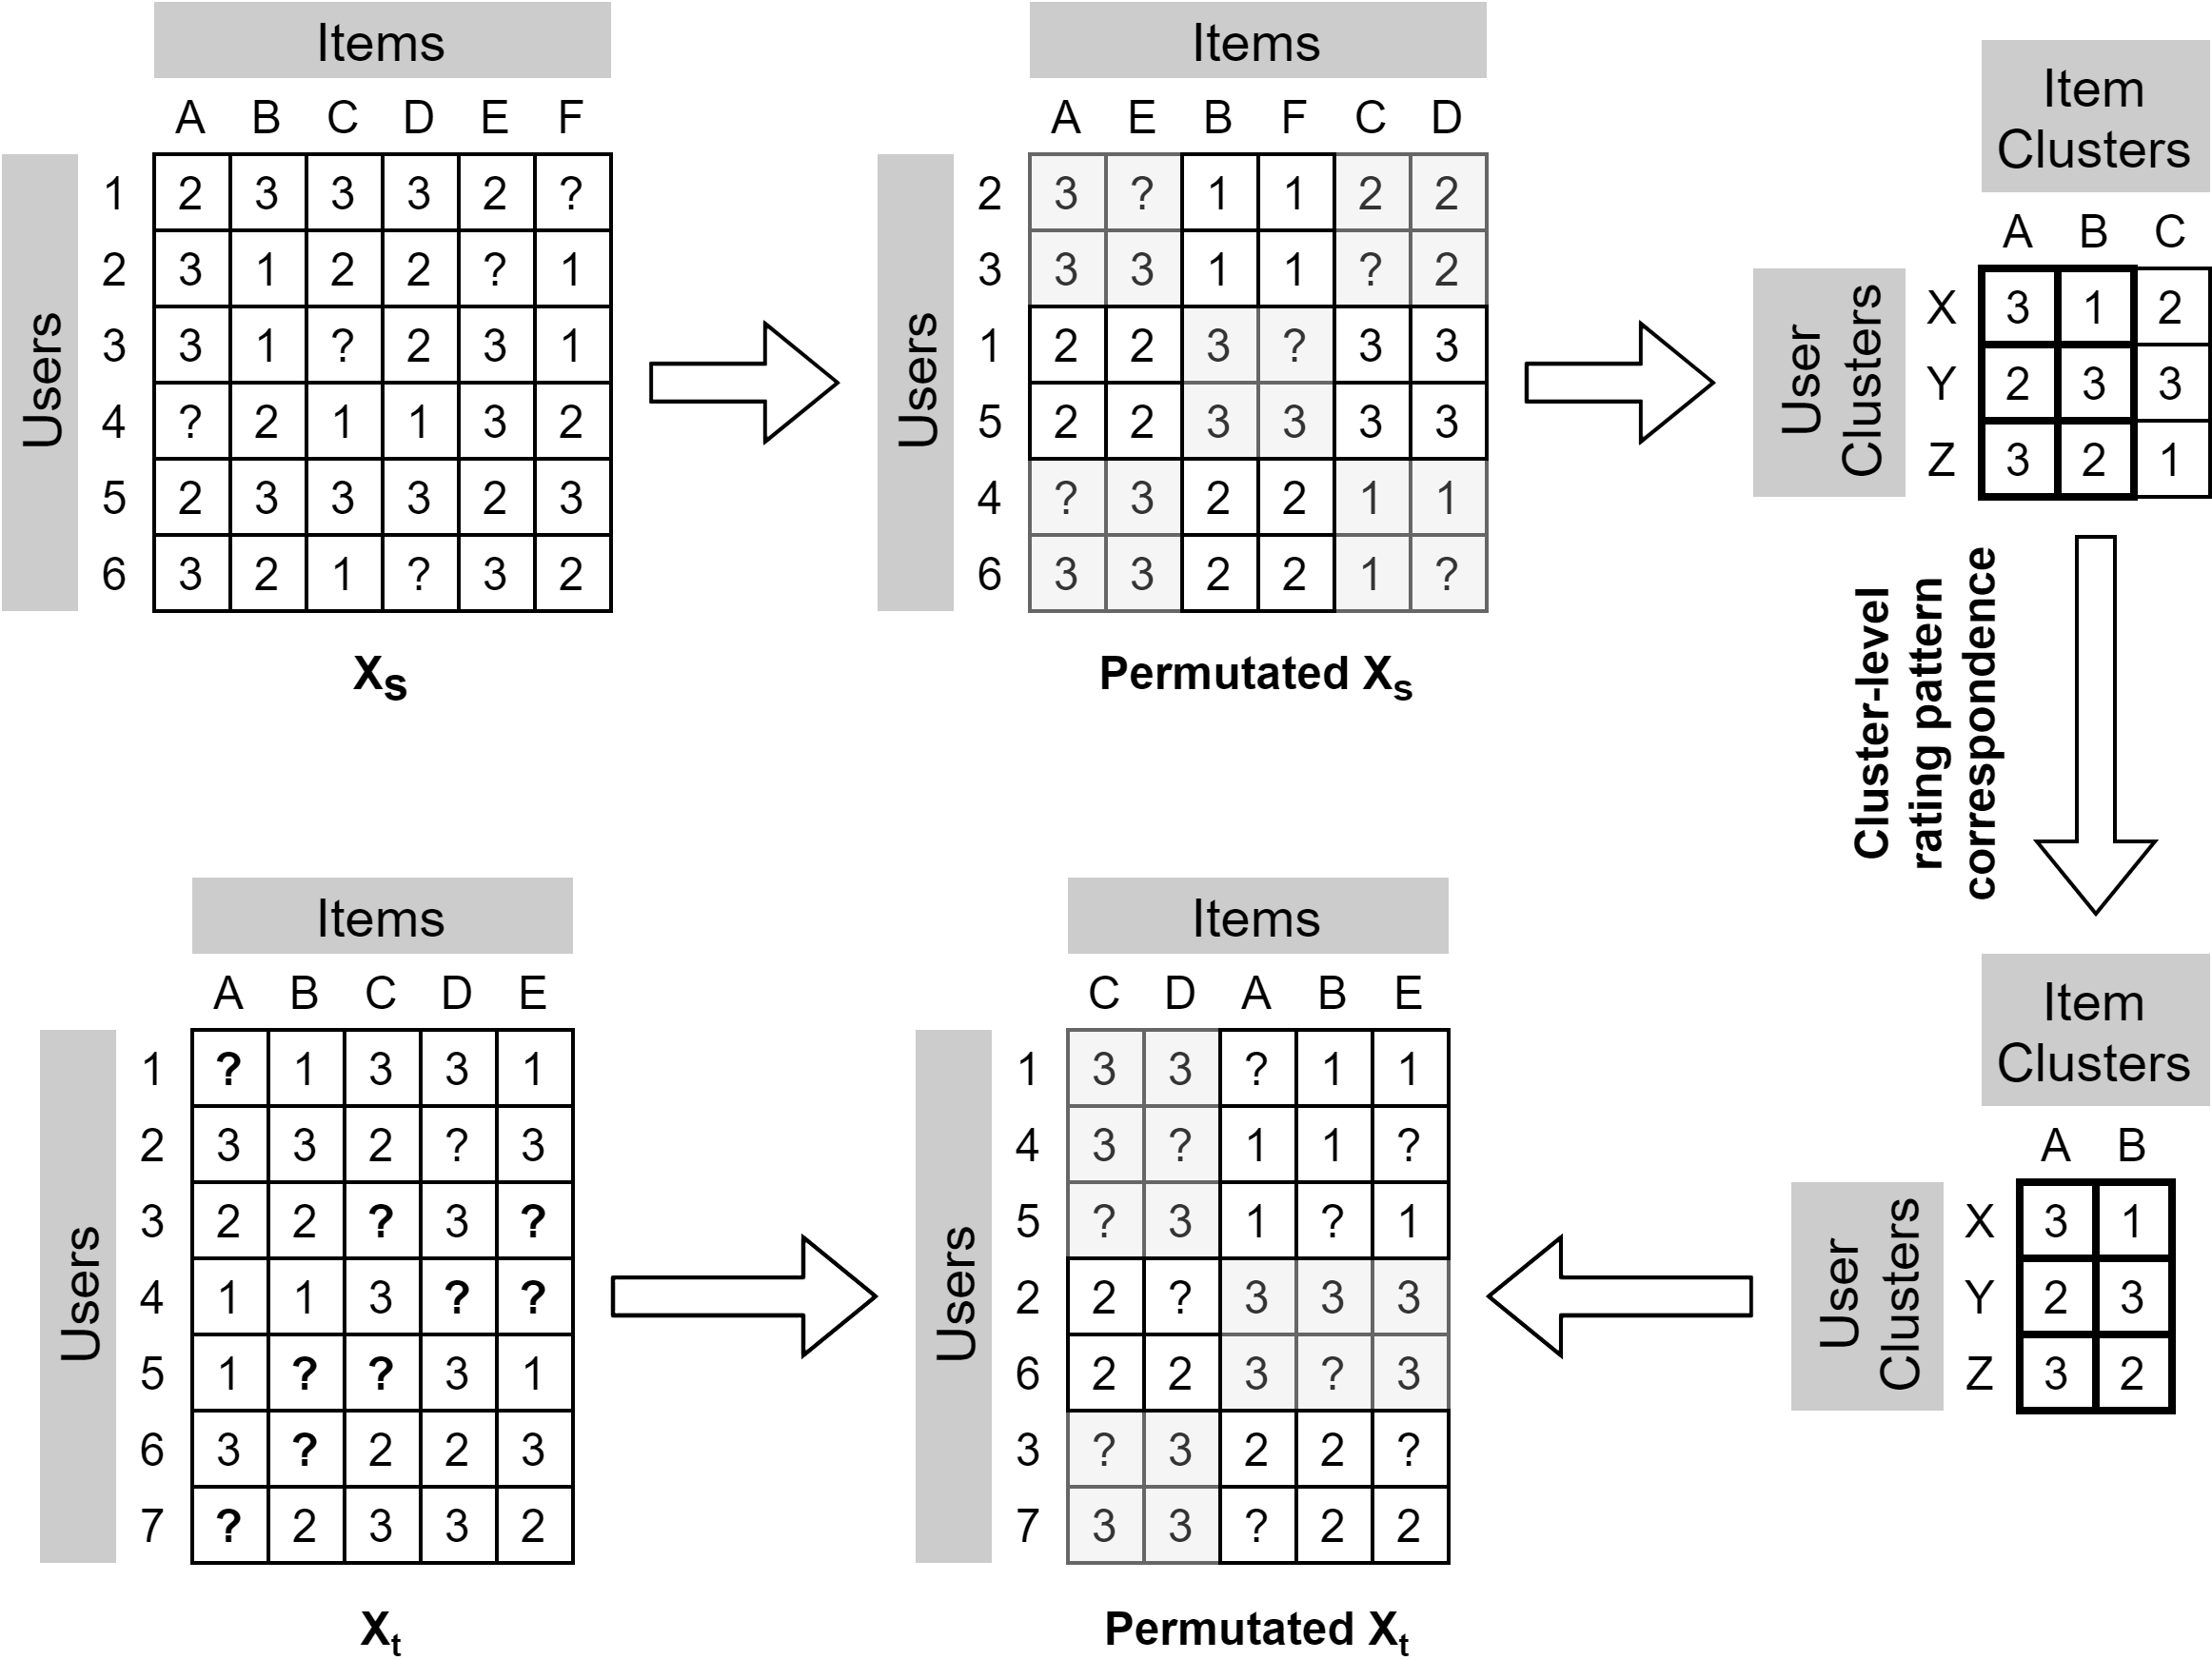
\includegraphics[width=0.8\textwidth]{pictures/codebook-construction}
  \caption{Example of codebook construction. Source: https://dl.acm.org/doi/10.5555/1661445.1661773}
\end{figure}


\subsection{Codebook Transfer}

Having constructed the codebook $B$, the model applies it to the target domain. To do this, it assumes that there is correspondence of user and item clusters between the two domains. Transferring the rating pattern consists in the inverse operation to codebook construction. The codebook is expanded to reconstruct an approximation of the target user-rating matrix $X_t$.\\
The duplication of a row or column of the codebook implies that there is a set of users or items in the target domain that behaves like the cluster represented by the row or column.\\
Once an approximation of $X_t$ has been obtained, it is suitable to exclude the already observed ratings in order to predict only the missing entries.\\
The minimization problem for codebook transfer is defined as follows:
\begin{equation}
\min_{U_t \in \{0,1\}^{p \times k}, V_t \in \{0,1\}^{q \times l}} \norm{[X_t - U_t B V_t^T] \odot W}^2_F, \quad \text{s.t.} \quad U_t 1 = 1, V_t 1 = 1
\end{equation}
where $U_t$ and $V_t$ are the matrices of cluster membership, respectively for users and items, such that:
\begin{equation}
  [U_t]_{ij} =
  \begin{cases}
    0, & \text{if user}\ [X_t]_{i}\ \text{belongs to cluster}\ j\\
    1, & \text{otherwise}
  \end{cases}
  , \quad \text{s.t.} \quad i \in \{1,p\}, j \in \{1,k\}
\end{equation}
\begin{equation}
  [V_t]_{ij} =
  \begin{cases}
    0, & \text{if item}\ [X_t]_{i}\ \text{belongs to cluster}\ j\\
    1, & \text{otherwise}
  \end{cases}
  , \quad \text{s.t.} \quad i \in \{1,q\}, j \in \{1,l\}
\end{equation}
and $W$ is the masking matrix with shape $p \times q$ such that:
\begin{equation}
  W_{ij} =
  \begin{cases}
    0, & \text{if}\ [X_t]_{ij}\ \text{is not rated}\\
    1, & \text{otherwise}
  \end{cases}
  , \quad \text{s.t.} \quad i \in \{1,p\}, j \in \{1,q\}
\end{equation}
The complete algorithm for codebook transfer is the following:
\vskip 0.7cm
\begin{algorithm}[H]
\SetKwInOut{Input}{Input}
\SetKwInOut{Output}{Output}
\Input{The codebook $B \in \mathbb{R}^{k \times l}$ learned from $X_s$;\\
The target domain user-rating matrix $X_t \in \mathbb{R}^{p \times q}$;\\
The masking matrix $W \in \{0,1\}^{p \times q}$.}
\Output{The filled target domain user-rating matrix $\bar{X_t}$.}
Allocate spaces for $U_s$ and $V_s$\;
\For{$i \gets 1$ \KwTo $m$}
{
  $\hat{j} =\ \text{random from}\ \{1,...,l\}$\;
  $[V^{(0)}_t]_{i\hat{j}} \gets 1$\;
  \For{$j \in (1,...,l)/\hat{j}$}
  {
    $[V^{(0)}_t]_{ij} \gets 0$\;
  }
}
\For{$t \gets 1$ \KwTo $max\_iteration$}
{
  \For{$i \gets 1$ \KwTo $p$}
  {
    $\hat{j} = argmin_j\norm{[X_t]_{i*} - [B [V^{(t - 1)}_t]^T]_{j*}}^2_{W_{i*}}$\;
    $[U^{(t)}_t]_{i\hat{j}} \gets 1$\;
    \For{$j \in (1,...,k)/\hat{j}$}
    {
      $[U^{(t)}_t]_{ij} \gets 0$\;
    }
  }
  \For{$i \gets 1$ \KwTo $q$}
  {
    $\hat{j} = argmin_j\norm{[X_t]_{*i} - {[U^{(t - 1)}_t B]}_{*j}}^2_{W_{*i}}$\;
    $[V^{(t)}_t]_{i\hat{j}} \gets 1$\;
    \For{$j \in (1,...,l)/\hat{j}$}
    {
      $[V^{(t)}_t]_{ij} \gets 0$\;
    }
  }
}

\caption{The algorithm for codebook transfer}
\end{algorithm}
\vskip 0.7cm
\begin{figure}[hbt!]
  \centering
  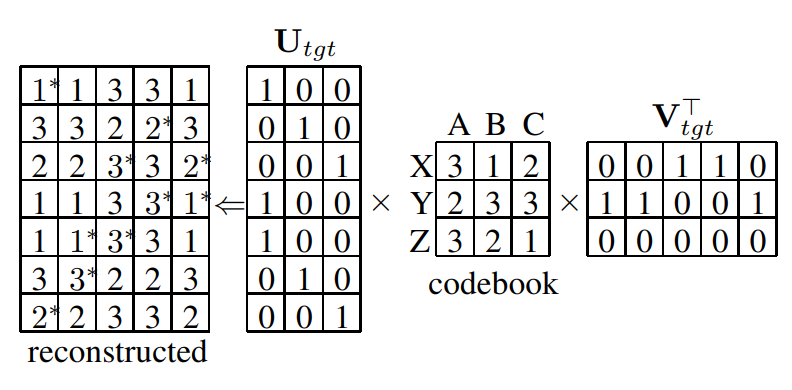
\includegraphics[width=0.8\textwidth]{pictures/codebook-transfer}
  \caption{Example of codebook transfer. Source: https://dl.acm.org/doi/10.5555/1661445.1661773}
\end{figure}


\subsection{Top-K Recommendations}



\section{LKT-FM}